
\chapter{April - 2012} % Chapter title

\label{ch:april:2012} % For referencing the chapter elsewhere, use \autoref{ch:introduction} 

%----------------------------------------------------------------------------------------
\section{Reading Game Theory}
Book name: {\it Fun and games, a text on game theory}

A game is being played whenever people interact with each other. What happens when people interact in {\bf a rational manner}

Those insects and plants whose genes programmed them to behave irrationally are now extinct.

We become distressed when confronted with {\bf circle reasoning}. But circle reasoning can not be evaded in considering strategic issues. 

Game theorists introduce their toy games with silly stories, which allow us to disengage our emotions from the problem.

\subsection{A example: One house, two bider}
Two bider: Horace and Maurice. 
The only way that Horace can be sure of keeping Maurice guessing, is by using a mixed strategy. What this means is that Horace should {\it \bf randomize} over the bids that it is sensible for him to make.

How should Horace randomize? For example, Never bid less than \$3 or more than \$ $3.5$.
If Horace seals \$b in his envelope,


{(\it 4.1 Payoffs)} Players act as though seeking to maximize the expected value of Von Neumann and Moregenstern utility function $u_i : \Omega \rightarrow \mathbb{R} $ defined on the set $\Omega$ of final outcomes of the game. Player $i$'s payoff at an outcome $\omega$ is then simply the Von Neumann and Moregenstern utility $u_i(\omega)$.
If the payoff $\phi$ includes a probability value, the game seems interesting.

{(\it 4.3 Matrices, 4.4 Vectors)} 

\subsection{2012-03-23}
rpc.rstatd is the dameon service of linux system information. The service collects such as CPU, system load and other information. If a client of rstat like rup or rsysinfo sends a request, the service will response the request. It is invoked by the system service xinetd. In addition, the service portmap provides the UDP output interface.  

\hfill {\tiny edited on 2012-04-29}

\section{Spell checking, Vim tips}
We should turn on the spell checking function in most of writing time.
\begin{enumerate}
\item Turn On:  \begin{center}\bf :set spell \end{center}
\item Turn Off:  \begin{center}\bf :set nospell \end{center}
\item Move the cursor to next wrong spelling:  \begin{center}\bf ]s \end{center}
\item Move the cursor to the previous wrong spelling:  \begin{center}\bf [s \end{center}
\item Add the user-defined word into the spell dictionary:  \begin{center}\bf zg \end{center}
\item Remove the user-defined word from the spell dictionary:  \begin{center}\bf uzg \end{center}
\item List all spelling recommendations about the wrong word:  \begin{center}\bf z= \end{center}
\item Set the spelling language:  \begin{center}\bf :set spelllang=en\_GB.UTF-8 \end{center}
\item Show the current spelling language:  \begin{center}\bf :echo \&spelllang  \end{center}
\end{enumerate}
\hfill {\tiny edited on 2012-04-27}

\section{Find and Replace, Vim tips}
\begin{enumerate}
\item The symbol {\bf \#} can be used for a separator, like the symbol {\bf /}. The following commands carry out the same functions.  
\begin{center}
35, 68 s/aaaa/bbbb/gc \\
35, 68 s\#aaaa\#bbbb\#gc
\end {center}
\end{enumerate}
\hfill {\tiny edited on 2012-04-27}

\section{Matrix, Matlab tips}
\label{sec:matlab}
\begin{enumerate}
\item Return every dimension of array $A$ in separate variables $m$ and $n$.  For example,
    $$[m,n] = \text{size}(A);$$
\item Return the $i$th row of array $A$ and the $j$th column of array $B$. For example,
    $$A(i,:);B(:,j);$$
\item {\bf Delete} the $i$th row of array $A$ and the $j$th column of array $B$. For example,
    $$A(i,:)=[\quad ]; B(:,j)=[\quad ];$$
\item Sum all values of elements in the $i$th column of array $A$. 
    $$\text{sum}(A(:,i))$$
\item Add a new row into array $A$ given that they have same column.
    $$A=[A;row];$$
\item Sum cumulatively the $j$th column of array $A$, 
    $$a = \text{cumsum}(A(:,j))$$
\item Clear the memory occupied by variables whose prefix is 'a', except the variable 'ab'.
    $$\text{clearvars a* -except ab};$$
\end{enumerate}
\hfill {\tiny edited on 2012-04-27}

\section{Moving smooth filter, Matlab}
When dealing with the data with plenty of samples, we use the tool, 'plot', to get the figure to show the trend of data.  If the interval of sampling is too small, the curve of samples seems to fluctuate drastically. It might cause the trouble that the trend not to be seen clearly. We use the tool, 'Moving Smooth filter' to handle the trouble.  
The function 
\begin{center}
$y$ = filter($b, a, x$)
\end{center}
creates the filtered data $y$ by processing the data in vector $x$ with the filter described by vectors $a$ and $b$.
The filter function is a general tapped delay-line filter, described by the difference equation, \autoref{eqn_moving_filter}.
\begin{align}
a(1)y(n) &= b(1)x(n) + b(2)x(n-1) + \cdots + b(N_b)x(n-N_b+1) \notag\\
& -a(2)y(n-1)- \cdots - a(N_a)y(n-Na+1)
\label{eqn_moving_filter}
\end{align}
\hfill {\tiny edited on 2012-04-29.}

\section{Plotting Figures, Default Values, Matlab}
Yesterday, I faced a problem about the default size of markers when I plotted a curve. After googled the content with the keywords 'default marker size', I got the information like this in the following:
For line objects, you can use
\begin{verbatim}
set(0,'DefaultLineMarkerSize',12);
set(0,'DefaultLineMarker','d');
set(0,'DefaultLineLineWidth', 2);
\end{verbatim}
Similarly, for axes objects, you can use these statements:
\begin{verbatim}
set(0,'DefaultAxesLineWidth', 2);
set(0,'DefaultAxesXGrid','on');
set(0,'DefaultAxesTickDir','out');
set(0,'DefaultAxesTickLength',[0.015 0.015]);
set(0,'DefaultAxesFontName','Arial')
\end{verbatim}
There are also two problems. One is that there are so many markers on curves that the figure seems unclear. I downloaded a tool called 'Nummarkers', which can set the number of makers shown on the curves. The other is that the gray figures with 'eps' format are not exported correctly. The tool 'ExportFig' can solve it. Note: the two tools can be download from the Matlab website.
\begin{verbatim}
h = plot(x,y1, x,y2);
nummarkers(h, 19, 1);

exportfig(h, strcat(main_dir_name,file_name,'.eps'), ... 
        'Format','eps', 'LockAxes', 1, 'Color', 'gray');
exportfig(h, strcat(main_dir_name,file_name,'.tif'), ...
        'Format','tiff', 'Resolution', 600, 'Color', 'rgb');
exportfig(h, strcat(main_dir_name,file_name,'.pdf'), ... 
    'Format', 'pdf', 'Color', 'rgb')
\end{verbatim}
\hfill {\tiny edited on 2012-04-29.}

\section{GSview}
GSview tool is used to view the EPS figures. The register codes are:
\begin{align*}
32411-26380\\
18963-21159\\
16417-30959
\end{align*}
\hfill {\tiny edited on 2012-04-29.}

\section{Beauty Face}
It is said that handsome faces have the two key ratio. The first one is the distance between two eyes to the distance between two ears. The second one is distance between eyes and mouth to the distance between chin and hair, shown in \autoref{fig:beauty_face}.
\begin{figure}
\begin{center}
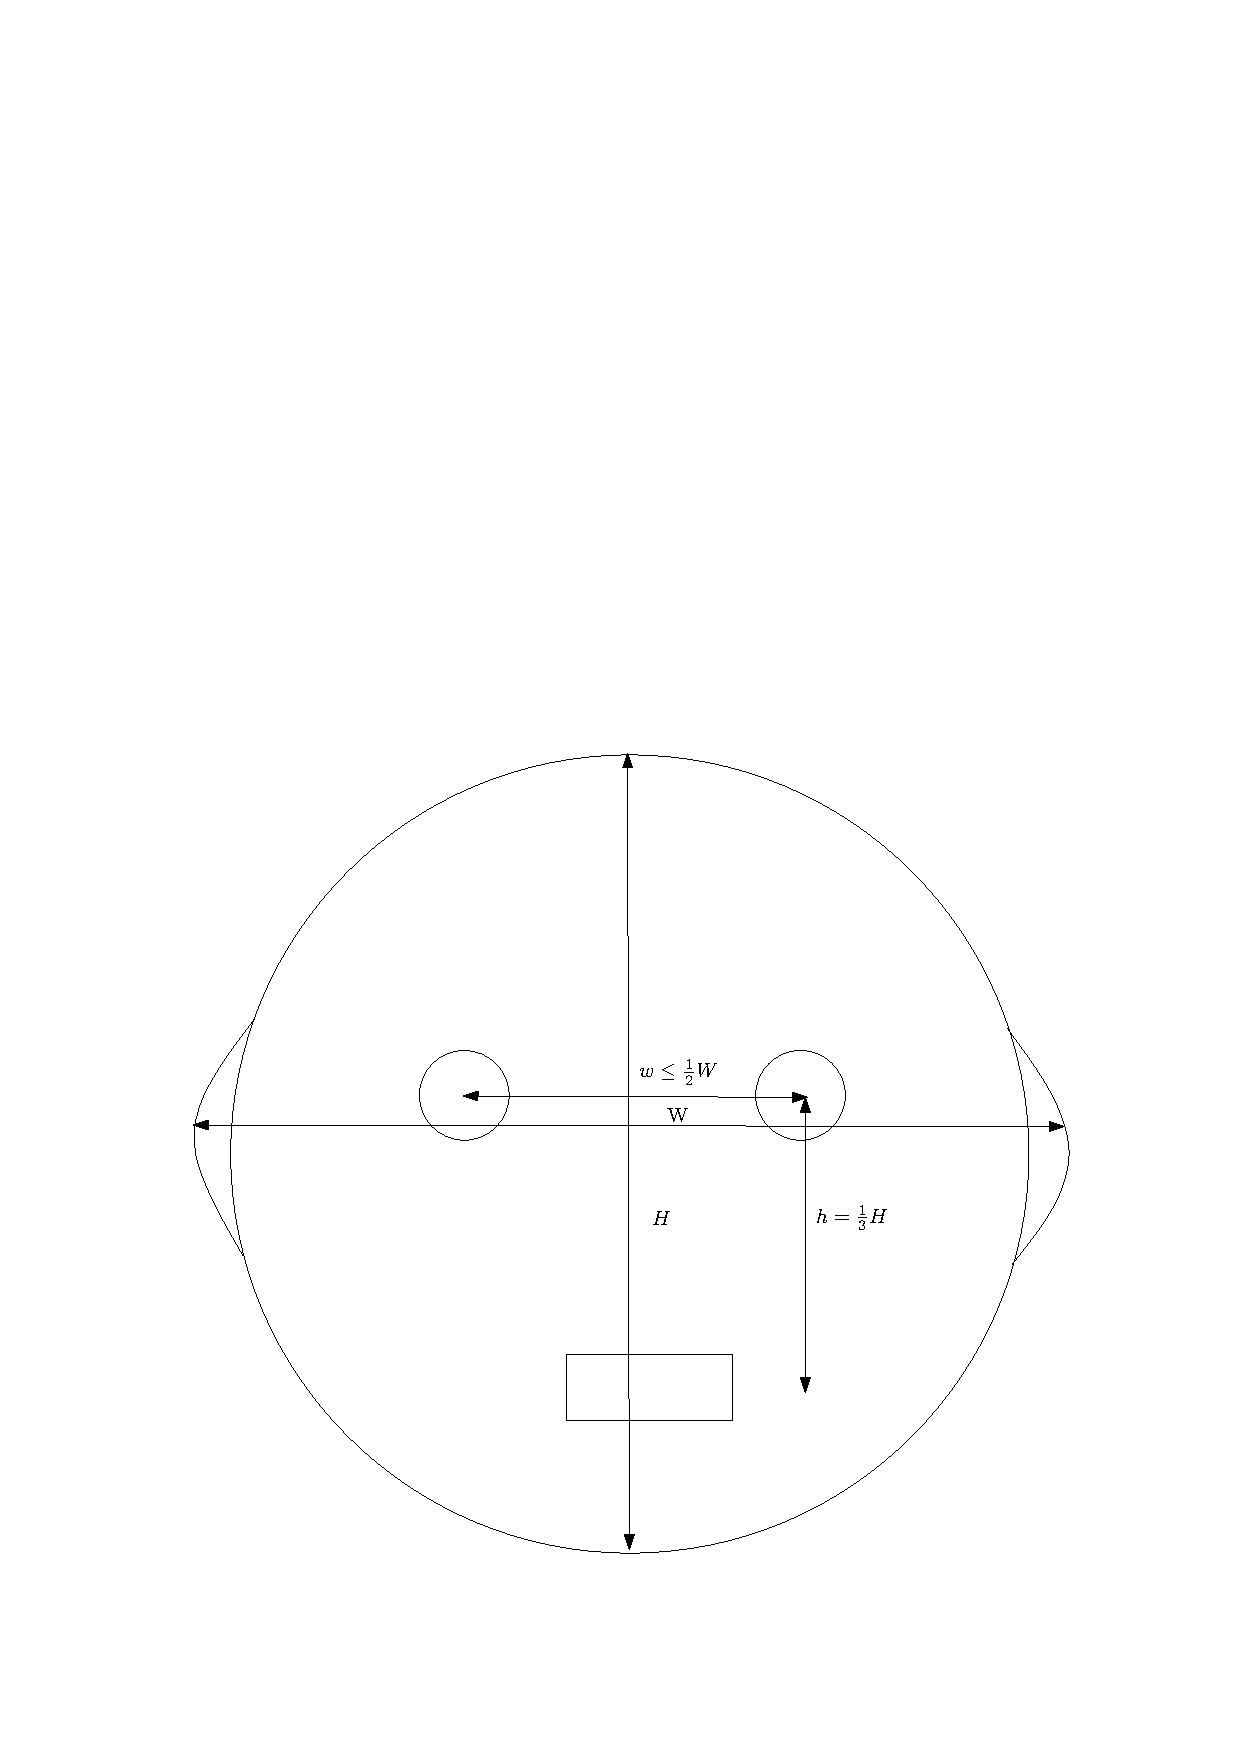
\includegraphics[width=.7\linewidth]{gfx/beauty_face}
\end{center}
\caption{The key ratios}
\label{fig:beauty_face}
\end{figure}
\hfill {\tiny edited on 2012-04-29.}

\section{Skype, China version}
If you make a call via the Skype-Tom Chinese version, you should add a symbol '*' before phone numbers. It looks like:
\begin{center}
*03733029531
\end{center}
\hfill {\tiny edited on 2012-04-30.}
\section{Git and Dropbox}
Today, I suddenly have a idea about backup of my important files. That method is to combine the Git and Drop-box. The Git system can deal with the version control. Drop-box automatically handles the backup operations on the remote server. The following steps are shown in detail here. We assume that the backup directory' name is "phd\_thesis", which includes several files, \texttt{"chapter01.doc"} and \texttt{"chapter01.bak"}. 
\begin{enumerate}
\item put a file named \texttt{'.gitignore'} into the root directory of 'phd\_thesis'. If we do not backup the file \texttt{'chapter01.bak'}, we insert its name into the \texttt{'.gitignore'} file. You have better add the names of ignored files into the file in advance. If the Git system have tracked the files, the complicated steps can remove them from the Git system.
\item Initialize Git on the working directory and files, like 
\begin{verbatim}
cd ~/phd_thesis
~/phd_thesis $ git init
~/phd_thesis $ git add .
~/phd_thesis $ git commit -m "first commit"
\end{verbatim}
\item Initialize Git on the Drop-box default directory, like
\begin{verbatim}
cd ~Dropbox/git
~/Dropbox/git $ git init --bare phd_thesis.git
\end{verbatim}
\item Sync the directories from local disk 'master' to drop-box 'phd\_thesis'.
\begin{verbatim}
~/phd_thesis $ git remote add phd_thesis 
                ~/Dropbox/git/phd_thesis.git
~/phd_thesis $ git push -u phd_thesis master
\end{verbatim}
\item Clone from the drop-box. 
\begin{verbatim}
Local clone:
    git clone  ~/Dropbox/git/phd_thesis.git
    git clone file://~/Dropbox/git/phd_thesis.git/chapter01.doc

Remote clone other computer's repository:
    git ssh://[user@]host.xz[:port]/path/to/repo.git/
    git git://host.xz[:port]/path/to/repo.git/
    git http[s]://host.xz[:port]/path/to/repo.git/
    git ftp[s]://host.xz[:port]/path/to/repo.git/
    git rsync://host.xz/path/to/repo.git/
\end{verbatim}
\end{enumerate}

\hfill {\tiny edited on 2012-04-30.}

\marginpar{Most people won't realize that writing is a craft. You have to take your appernticeship in it like anything else. \\
-Katherine Anne Porter}
%%%%%%%%%%%%%%%%%%%%%%%%%%%%%%%%%%%%%%%%%%%%%%%%
